\chapter{Suspended material transport by tidal straining
  near sloping topography}
\label{kap-slope}

To investigate basin scale sediment transport pathways, a knowledge 
about the underlying, small scale processes is crucial. Motivated by the 
outcome of studies on estuarine dynamics controlling sediment transport 
processes, a basic process study describing the impact on sediment transport of 
an oscillatory current moving over sloping topography is discussed in the 
following. Parts of the following chapter were published in 2016 in the Journal 
of Physical Oceanography under the title "Residual transport of suspended 
material by tidal straining near sloping topography".

Tidal straining is known to have an important impact on the
  generation of residual currents and the transport of suspended
  material in estuaries and the coastal ocean. Essential for this
  process is an externally imposed horizontal density gradient,
  typically resulting from either freshwater runoff or differential
  heating. Here, we show that near \emph{sloping} topography, tidal
  straining may effectively transport suspended material across
  isobaths even if freshwater runoff and differential heating do not
  play a significant role. A combined theoretical and idealized
  modeling approach is used to illustrate the basic mechanisms and
  implications of this new process. The main finding of this study is
  that, for a wide range of conditions, suspended material is
  transported upslope by a pumping mechanism that is in many respects
  similar to classical tidal pumping. Downslope transport may also
  occur, however, only for the special cases of slowly sinking
  material in the vicinity of slopes with a slope angle larger than a
  critical threshold. The effective residual velocity at which
  suspended material is transported across isobaths is a significant
  fraction of the tidal velocity amplitude (up to 40\% in some cases),
  suggesting that suspended material may be transported over large
  distances during a single tidal cycle. \citep{schulzumlauf2016}

\section{Introduction\label{sec:intro}}
Subtidal circulation and residual transport of suspended material in
estuaries and the coastal ocean is known to be tightly connected to
the presence of horizontal density gradients, generated by either
river runoff, differential heating, or differential evaporation. The
most obvious dynamical implication of such horizontal density
differences is the generation of a gravitationally-driven residual
circulation with a landward transport of dense waters near the bottom,
and a seaward return current above
\citep{Pritchard1952,MacCreadyGeyer2010}.

Residual currents may also be triggered by periodic variations of
stratification induced by the oscillatory vertical shear of a tidal
flow acting on the horizontal density gradient. This mechanism leads
to a periodic ``tidal straining'' of the horizontal density gradient
\citep{Simpsonetal90a}, resulting in weak or even convectively
unstable stratification during flood, and therefore in significantly
larger turbulent diffusivities compared to the more stably stratified
ebb period (\fig{straining}a,c). 
\begin{figure}[h]
  \noindent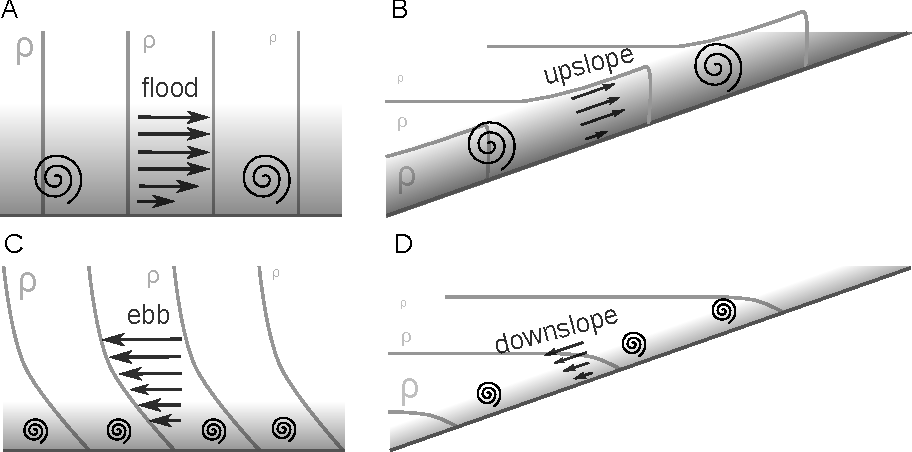
\includegraphics[width=30pc,angle=0]{bilder/geometryvergleich.pdf}\\
  \caption{Sketch of density structure during tidal straining (a,c) in
    an estuary or a region of fresh water influence, and (b,d) near
    sloping topography. Arrows show the instantaneous currents;
    suspended material is indicated by the gray-shaded areas near the
    bottom.}\label{straining}
\end{figure}

\cite{JayMusiak94a} proposed that
this tidal asymmetry in turbulent mixing may have a profound impact on
the tidally averaged momentum budget. They pointed out that the
stronger vertical homogenization of momentum during the more turbulent
flood phase leads to a residual current that augments the
gravitationally-driven residual circulation
\citep[see][]{MacCreadyGeyer2010}. Exploring the physically relevant
parameter space with a one-dimensional numerical model,
\cite{BurchardHetland2010a} concluded that the residual circulation
due to tidal straining typically dominates over the gravitational
circulation in tidally energetic environments.

Whereas the residual circulation described above largely determines
the horizontal transport of dissolved substances, additional effects
have to be considered when modeling the residual transport of
suspended particulate matter (SPM) with a sinking motion relative to
the moving fluid. During the more turbulent flood phase
(\fig{straining}a), SPM concentrations are typically larger due to
enhanced erosion, and suspended material is mixed up higher into the
water column compared to the less turbulent ebb phase
(\fig{straining}c). The correlation between these asymmetries in
concentration and the oscillating current results in a ``tidal
pumping'' mechanism that induces a net landward transport of suspended
material
\citep{Unclesetal85a,JayMusiak94a,ScullyFriedrichs2007a}. Using a
one-dimensional coupled sediment transport model,
\cite{Burchardetal2013a} showed that, for a broad range of parameters,
tidal pumping is much more effective in transporting suspended
material compared to advection by the residual current. This finding
is in line with \cite{ScullyFriedrichs2003a}, who pointed out that the
transport due to tidal straining may even adverse the residual
advective transport.

A related periodic straining process, not requiring any externally
imposed horizontal density gradients, has recently been identified
near the slopes of stratified lakes \citep{Lorkeetal2005a}. In this
case, a cross-slope (i.e., an approximately horizontal) density
gradient is generated by the projection of the purely vertical
interior stratification onto the sloping topography of the lateral
boundaries of the basin (\fig{straining}b,d). In the presence of
oscillating up- and downslope currents, associated with basin-scale
internal-wave motions in the case studied by \cite{Lorkeetal2005a}, a
shear-induced straining of the cross-slope density gradient is
observed, analogous to classical tidal straining. During upslope flow,
dense water is advected on top of lighter near-bottom water, leading
to a reduction of vertical stratification, and ultimately to
convection (\fig{straining}b). Vice-versa, during periods of downslope
flow, stable stratification evolves due to the downslope advection of
lighter water on top of denser near-bottom fluid, resulting in a
suppression of turbulent mixing (\fig{straining}d). This effect has
been observed in lakes of different size and geometry
\citep{Lorkeetal2005a,Lorkeetal2008a,CossuWells2013a}, and could be
reproduced in three-dimensional numerical modeling studies
\citep{BechererUmlauf2011a,Lorraietal2011a}. A recent study by
\cite{Endohetal2016a} provided first direct observational evidence for
the occurrence of slope-induced tidal straining on the continental
shelf, and suggested that this process may also be important for the
cross-slope transport of suspended material.

\cite{UmlaufBurchard2011a} used an idealized one-dimensional numerical
model to study the relevance of these findings for the
oceanographically relevant parameter space. Their simulations revealed
that shear-induced periodic stratification (SIPS) in sloping BBLs is
expected to occur for virtually any parameter constellation, and
triggers a residual circulation that is in many respects similar to
classical tidal straining. The transport of suspended material was,
however, not investigated in this study.

In view of these similarities, and relevance of classical tidal
straining for the transport of suspended material in estuaries and the
coastal ocean, it would be interesting to understand under which
conditions and by which mechanisms tidal straining near sloping
topography may be able to transport suspended material across
isobaths. Here, we investigate this question with the help of a
combined theoretical and idealized modeling approach, focusing on the
identification of the basic mechanisms that determine cross-isobath
transport of suspended material. The model, described in detail in
Section \ref{sec:geometry}, builds up on the model by
\cite{UmlaufBurchard2011a}, extended here by adding a simple erosion
and transport model for suspended material. In Section \ref{sec:bbl},
we investigate the basic SPM transport mechanisms due to tidal
straining near sloping topography with the help of a few idealized
examples. The relevant (non-dimensional) parameters are identified in
Section \ref{sec:nondim}, and the parameter space is then explored in
Section \ref{sec:results} before we draw some conclusions in Section
\ref{sec:conclusions}.


\section{Geometry and governing equations\label{sec:geometry}}

\subsection{Geometry}
\begin{figure}[h]
  \noindent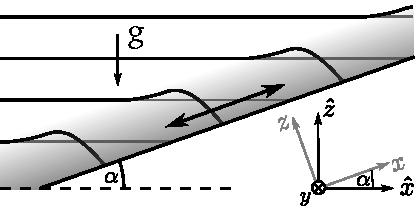
\includegraphics[width=19pc,angle=0]{bilder/geometry.pdf}\\
  \caption{Schematic view of isopycnal structure (black lines) in
    the vicinity of a uniform plane slope with slope angle
    $\alpha$. Suspended material is indicated by the gray-shaded
    region near the bottom. The double arrow indicates the oscillatory
    current up and down the slope, the gray lines show the equilibrium
    levels of the isopycnals. The upslope and slope-normal coordinates
    are denoted by $x$ and $z$, respectively.}\label{slopesketch}
\end{figure}
We investigate the motion of a Boussinesq fluid in a semi-infinite
domain bounded by a uniform slope with slope angle $\alpha$
(\fig{slopesketch}). For simplicity, we ignore the effects of rotation, and
assume that the geometry is two-dimensional with the horizontal and
vertical coordinates referred to as $\hat{x}$ and $\hat{z}$,
respectively. Vertical stratification is quantified with the help of the
squared buoyancy frequency,
\begin{equation}
  \label{NN}
  N^2 = \partder{b}{\hat{z}} \comma
\end{equation}
where $b$ denotes the buoyancy of the fluid (all quantities are
Reynolds-averaged unless noted otherwise). Outside the BBL, we assume
that $b$ approaches the undisturbed equilibrium buoyancy $b_\infty$,
which is characterized here by strictly horizontal isopycnals (gray
lines in \fig{slopesketch}) and constant stratification:
\begin{equation}
  \label{NNinf}
  N^2_\infty = \partder{b_\infty}{\hat{z}} \point
\end{equation}
It should be noted that, although $N_\infty$ is constant by
definition, $b_\infty$ may vary in space and time due to up- and
down-slope advection as discussed in more detail below.

\cite{UmlaufBurchard2011a} showed that this two-dimensional problem
can be reduced to one dimension by introducing the rotated upslope and
slope-normal coordinates $x$ and $z$ ($z=0$ at the bottom), and assuming that all upslope
gradients except the buoyancy gradient vanish (see \fig{slopesketch}). Under
these conditions, it is easy to show that the upslope buoyancy
gradient is constant, and given by
\begin{equation}
  \label{dbdx}
    \partder{b}{x} = N^2_\infty \sin \alpha  
    \point
\end{equation}
The slope-normal buoyancy gradient is defined as
\begin{equation}
  \label{NNcheck}
   \check{N}^2  = \partder{b}{z} \comma 
\end{equation}
which does not depend on $x$, and converges to
\begin{equation}
 \label{NNinfconv}
 \check{N}^2 = N^2_\infty \cos \alpha \quad \text{for} \quad z
 \rightarrow \infty \comma
\end{equation}
far away from the bottom and thus outside the BBL.

\subsection{Equations of motion}
Starting from the Reynolds-averaged Boussinesq equations,
\cite{UmlaufBurchard2011a} showed that under the above assumptions,
the equations of motion can be expressed as
\begin{equation}
  \label{ub}
  \begin{array}{rcl}
    \partder{u}{t}
    &=& 
      (b - b_\infty) \sin \alpha + \partder{u_\infty}{t}
    - \partder{\tau}{z}                                    \comma \\[5mm]
    \partder{b}{t}
    &=& 
     - u N^2_\infty \sin \alpha
     - \partder{G}{z}                                      \comma \\[5mm]
  \end{array}
\end{equation}
where $t$ denotes time, $u$ the cross-slope velocity, $\tau$ the
slope-normal turbulent flux of momentum (normalized by some reference
density $\rho_0$), and $G$ the slope-normal turbulent buoyancy
flux. The latter two are defined as
\begin{equation}
  \label{fluxes}
  \begin{array}{rcl}
    \tau
    &=& 
    \overline{u^\prime w^\prime}
    = - \nu_t \partder{u}{z}                                \comma \\[5mm]
    G
    &=& 
      \overline{w^\prime b^\prime}
    = - \nu_t^b \partder{b}{z}                              \comma \\[5mm]
  \end{array}
\end{equation}
where the primes indicate turbulent fluctuations, and the overbar the
Reynolds average ($w$ is the slope-normal velocity). The turbulent
diffusivities of momentum and buoyancy, $\nu_t$ and $\nu_t^b$, are
computed from a second-moment turbulence closure model with two
transport equations for the turbulent kinetic energy $k$ and the
turbulence dissipation rate $\varepsilon$
\citep[see][]{UmlaufBurchard2005a}. We assume high Reynolds numbers,
and therefore ignore the molecular fluxes of momentum and buoyancy in
\eq{ub}. The turbulence model and all model parameters are identical
to the model used in \cite{UmlaufBurchard2011a} and
\cite{Umlaufetal2015a}, where a more detailed model description may be
found.

The term $\partial {u_\infty}\slash \partial t$ appearing in \eq{ub}
is an integration constant that, in general, depends on time, and
plays the role of a prescribed external pressure gradient used to
force the model. Internal pressure gradients are represented by the
term $(b - b_\infty) \sin \alpha$, which mirrors the tendency of
isopycnals to relax back towards their equilibrium levels (see
\fig{slopesketch}). The equilibrium buoyancy $b_\infty$ is computed
from an evolution equation of the form
\begin{equation}
  \label{equib}
  \partder{b_\infty}{t} + u_\infty N_\infty^2 \sin \alpha = 0
  \comma
\end{equation}
which represents the up- or downslope advection of the undisturbed
buoyancy field \citep{UmlaufBurchard2011a}.

At the lower boundary, we use a no-slip condition for the velocity,
and assume that the buoyancy flux vanishes:
\begin{equation}
  \label{bound}
  \begin{array}{rcl}
    u
    &=& 
    0 \comma  \\[5mm]
    \partder{b}{z} &=&	 0                                 \point \\[5mm]
   \end{array}
\end{equation}
Boundary conditions for the turbulence quantities are discussed in
\cite{UmlaufBurchard2011a}, who assumed that the bottom is
hydrodynamically rough (which introduces the bottom roughness $z_0$ as
an additional external parameter), and that a logarithmic wall-layer
exists very close to the bottom. Far away from the lower boundary ($z
\rightarrow \infty$), boundary conditions are derived from the
assumptions that $u$ and $N$ are uniform, and that all turbulent fluxes
vanish.

Assuming that there are no hydrodynamic feedbacks resulting from the
suspended material, equations \eq{ub} and \eq{equib} fully describe
the evolution of the unknowns $u$, $b$, and $b_\infty$. This system of
equations has been numerically solved for different parameters, using
a time step and grid size small enough to exclude any significant
numerical errors. Mathematical and numerical implementation details
are described in \cite{Umlaufetal2005a}.

\subsection{Boundary-layer forcing and resonance}
We restrict our analysis to the special case of an oscillatory outer flow,
\begin{equation}
  \label{uinfty}
  u_\infty = U \sin \omega t
  \comma
\end{equation}
where $U$ is the fixed velocity amplitude, $\omega=2 \pi /T_f$ the
forcing frequency, and $T_f$ the forcing period. Here, we focus
exclusively on motions at the $M_2$ tidal frequency ($T_f=12.4$~h)
such that $u_\infty$ provides a simple representation of the
near-bottom currents induced by barotropic or baroclinic tides.

\cite{UmlaufBurchard2011a} showed that BBL motions relative to the
interior contain both kinetic and potential energy, which suggests the
possibility of reversible BBL oscillations. It can be shown that these
oscillations occur at the frequency
\begin{equation}
  \label{omegac}
  \omega_c = N_\infty \sin \alpha
  \comma
\end{equation}
which happens to coincide with the frequency for the critical
reflection of internal waves impinging on a slope with slope angle
$\alpha$ \citep[see][]{Thorpe2005a}. Close to resonant forcing
($\omega \approx \omega_c$), it is therefore likely that the geometric
assumptions outlined above break down, and the model can no longer be
applied \citep{UmlaufBurchard2011a}. We therefore exclude this parameter 
range from the following analysis, and only consider the cases
$\omega \gg \omega_c$ (strongly supercritical forcing) and $\omega \ll
\omega_c$ (strongly subcritical forcing). Note that for given forcing
frequency $\omega$, \eq{omegac} may be inverted to compute the
critical slope angle, $\alpha_c$. Evidently, supercritical forcing
corresponds to subcritical slopes, and vice-versa.


\subsection{Erosion and transport of suspended material}

Focusing on the basic physical mechanisms determining the
transport of suspended material near sloping topography, we use a
relatively simple erosion and transport model. Suspended material is
assumed to sink vertically down with a constant settling velocity
$w_s$ but is otherwise considered to behave like a passive tracer (no
hydrodynamical feedbacks). Processes like aggregation or
disintegration of suspended particles are ignored. The evolution
equation for the concentration $c$ of suspended material is thus of
the form
\begin{equation}
  \label{c}
     \partder{c}{t} 
     = - \partder{}{z}\left( F_z -  c w_s \cos \alpha \right) 
     \comma
\end{equation}
where the slope-normal turbulent sediment flux is defined as
\begin{equation}
  \label{Fz}
  F_z = -\nu_t^b \partder{c}{z}
  \point
\end{equation}
Clearly, the cross-slope advection term $\partial (uc) / \partial x$
does not appear in \eq{c} due to the assumed cross-slope homogeneity
in our geometry. This assumption is formally valid only if the
length-scale $L_c$ of cross-slope variations in SPM concentration is
much larger than the tidal excusion scale: $L_c \gg U/T_f$. The
concentration of suspended material, however, may vary on smaller
scales in many situations, which should be kept in mind when
interpreting the results from this study.

At the lower boundary, the turbulent SPM flux $F_z$ in \eq{Fz} equals
the erosion flux, here determined from the classical expression
\begin{equation}
  \label{defFz}
  F_z = \alpha_e \max \left\{ \frac{\left| \tau_b \right| }{\tau_c} -1 , 0 \right\}
  \quad \text{for} \quad z=0,
\end{equation}
where $\alpha_e$ is the erosion coefficient, $\tau_b$ the
bottom shear stress, and $\tau_c$ the critical shear stress for
resuspension, both normalized by the constant reference density
$\rho_0$ \citep[see][]{krone1962,sanford1997,amoudry2011}. The
availability of erodible material is assumed to be unlimited in this
idealized study.

Note that, in general, the SPM parameters appearing in \eq{c} and
\eq{defFz} are not independent. E.g., for the relatively simple case
of non-cohesive material, \cite{vanRijn84b} suggests a relation
between $w_s$, $\tau_c$, and the grain size. The situation becomes,
however, considerably more complex if unsorted or non-cohesive
material is considered \citep[e.g.,][]{dade1992,sassi2015}, or if
biological activity (bioturbation, biofilms) play a significant role
\citep[][]{grant1986b,grant1994}. Because a generally valid relation is
not available at the moment, we consider $w_s$, $\tau_c$, and
$\alpha_e$ as independent parameters in our study. The physically
relevant range for these parameters is explored in detail in Section
\ref{sec:results}.

\subsection{Residual transports}
In order to quantify the tidally-averaged transport of SPM, we define
the total cross-slope residual flux,
\begin{equation}
  \label{Fx}
  F_x  = \mean{uc} - \mean{c} w_s \sin \alpha \comma
\end{equation}
where the angular brackets denote the tidal average. The last term in
\eq{Fx} is recognized as the projection of the vertical sinking
velocity onto the downslope direction. For the small slope angles
considered here, however, this ``sinking flux'' is negligible, and
will therefore be ignored in the following.

Following \cite{Burchardetal2013a}, we further decompose the residual
flux into contributions from the residual current and the tidal
fluctuations:
\begin{equation}
  \label{splitflux}
   \mean{uc} = \mean{u} \mean{c}  
             + \mean{ \tilde{u} \tilde{c} }
             \comma
\end{equation}
where the tilde indicates deviations from the tidal average. The first
term on the right hand side in \eq{splitflux} represents the
contribution of the residual current to the total residual flux,
whereas the second term, referred to as the ``tidal pumping'' term in
the following, mirrors the effect of tidal straining. Dividing
\eq{splitflux} by the average concentration $\mean{c}$, we find an
expression of the form
\begin{equation}
  \label{uc}
   u_c = \mean{u} 
             + \dfrac{ \mean{ \tilde{u} \tilde{c} } }{\mean{c}}
             \comma
\end{equation}
which may be interpreted as the effective velocity at which suspended
material is transported across the slope. Note from \eq{uc} that the
transport velocity $u_c$ may be significantly different from the
residual velocity $\mean{u}$ (both may even have opposite sign) if
tidal pumping is important.

\section{Boundary-layer dynamics and sediment transport\label{sec:bbl}}

As an example to illustrate the basic processes, we consider in the
following a case with a relatively mild slope ($\alpha=0.002$), a
typical tidal velocity amplitude ($U=0.5$~m~s$^{-1}$), and some other
typical parameters summarized in \tab{params} (Case 1). 
\begin{table}[h]
\caption{Parameters used for the simulation discussed in section
  \ref{sec:bbl}. Note that supercritical forcing corresponds to
  subcritical slopes, and vice-versa.}\label{params}
\begin{center}
\begin{tabular}{cccccc}
%\hline\hline
case  & forcing & $U$ & $\omega$ & $z_0$ & $\alpha_e$ \\
\hline
1 & supercritical & $0.5 \, \text{m s}^{-1}$ & $1.41 \times 10^{-4} \, 
\text{s}^{-1}$ & 
$10^{-2}\,\text{m}$ & $10^{-4} \, \text{kg 
s}^{-1}\text{ m}^{-2}$  \\
\hline
2 & subcritical & $0.5 \, \text{m 
s}^{-1}$ & $1.41 \times 
10^{-4} \, 
\text{s}^{-1}$ & 
$10^{-2}\,\text{m}$ & $10^{-4} \, \text{kg 
s}^{-1}\text{ m}^{-2}$\\
\hline
3 & subcritical & $0.5 \, \text{m 
s}^{-1}$ & $1.41 \times 
10^{-4} \, 
\text{s}^{-1}$ & 
$10^{-2}\,\text{m}$ & $10^{-4} \, \text{kg 
s}^{-1}\text{ m}^{-2}$\\
%\hline
\end{tabular}
\newline
\begin{tabular}{cccccc}
%\hline\hline
case & forcing & $\tau_c$ & $w_s$ & 
$N^2_\infty$ & 
$\alpha$ \\
\hline 
1 & supercritical & $10^{-4} \, \text{m}^2 \text{s}^{-2}$ & $5 \times 10^{-3}\,\text{m s}^{-1}$ & 
$10^{-4}\,\text{s}^{-2}$ & $2 \times 10^{-3}$ \\
\hline
2 & subcritical & $10^{-4} \, \text{m}^2 \text{s}^{-2}$ & $2 \times 
10^{-4}\,\text{m s}^{-1}$ & 
$10^{-3}\,\text{s}^{-2}$ & $5 \times 10^{-2}$\\
\hline 
3 & subcritical & $10^{-4} \, \text{m}^2 \text{s}^{-2}$ & 
 $9 \times 10^{-4}\,\text{m s}^{-1}$  & 
$10^{-3}\,\text{s}^{-2}$ & $5 \times 10^{-2}$\\
%\hline
\end{tabular}
\end{center}
\end{table}

According to
\eq{omegac}, in this example the resonance period of the BBL is $T_c =
2 \pi \omega_c^{-1} \approx 87$~h and the critical slope $\alpha_c
\approx 0.014$, indicating that tidal forcing is strongly
supercritical. Correspondingly, the slope is strongly subcritical. All
results discussed here and in the following sections correspond to
fully periodic conditions.

\subsection{Boundary-layer dynamics\label{sec:examp}}

As the sediment model has no feedback on the hydrodynamic part of the
problem, the evolution of the near-bottom velocities, stratification,
and mixing parameters is qualitatively similar to that discussed in
\cite{UmlaufBurchard2011a}. Here, we only briefly summarize the main
hydrodynamical characteristics of this type of flow to provide the
context for the following discussion of resuspension and residual SPM
transports.
\begin{figure}[h]
  \noindent\includegraphics[width=36pc,angle=0]{bilder/pannel.pdf}\\
  \caption{Temporal variability of (a) velocity, (b) magnitude of the
    squared buoyancy frequency, (c) turbulent diffusivity, (d) SPM
    concentration, and (e) magnitude of the bottom shear stress
    (black), critical shear stress for re-suspension (gray), and
    integrated sediment concentration (blue). Gray lines in panels
    (a)--(d) indicate gravitationally unstable regions. All results
    represent fully periodic conditions (time refers to the start of
    the simulation). Parameters correspond to Case 1 in
    \tab{params}. }\label{pannelgrafik}
\end{figure}

\fig{pannelgrafik}a,b shows that, for the parameters compiled in
\tab{params}, the oscillating tidal currents generate a BBL of
approximately 40~m thickness, characterized by strongly reduced
stratification below a sharp pycnocline that separates the BBL from
the non-turbulent interior region. During periods of upslope flow, a
large fraction of the BBL becomes gravitationally unstable (light gray
lines in \fig{pannelgrafik}), whereas during downslope flow it remains
stably stratified throughout. \cite{UmlaufBurchard2011a} showed that
the periodic destabilization of the BBL can be explained by a
differential advection mechanism resulting from the interaction of the
frictional near-bottom shear and the constant upslope density
gradient, analogous to tidal straining. More specifically, they showed
that during upslope flow, dense fluid may be transported on top of the
lighter, more slowly moving fluid in the immediate vicinity of the
bottom, resulting in unstable stratification, and thus turbulent
convection. It is worth noting that \cite{Endohetal2016a} reported
recent observations of this processes for a tidal BBL of similar
vertical scale on a sloping continental shelf.

The periodic changes in stratification visible in \fig{pannelgrafik}b
are directly mirrored in the turbulent diffusivities shown in
\fig{pannelgrafik}c. During periods of upslope flow, when weak or
unstable stratification develops, diffusivities are strongly enhanced
compared to the stratified period with downslope flow. This
variability in $\nu_t^b$ caused by tidal straining induces a tidal
asymmetry that is, besides gravitational forcing, the key trigger for
residual cross-slope transports inside the BBL.

SPM properties shown in \fig{pannelgrafik}d,e are consistent with
these tidal asymmetries in mixing. During periods of upslope flow, a
larger amount of material is resuspended (\fig{pannelgrafik}e), SPM is
mixed up higher into the water column, and SPM concentrations are
somewhat larger compared to periods with downslope flow
(\fig{pannelgrafik}d). These asymmetries can be interpreted as a
consequence of the larger turbulent diffusivities during upslope flow,
and the larger bottom shear stress, which, according to \eq{defFz}
determines the resuspension of settled material.


\subsection{Residual results\label{sec:trans}}
\begin{figure}[h]
  \noindent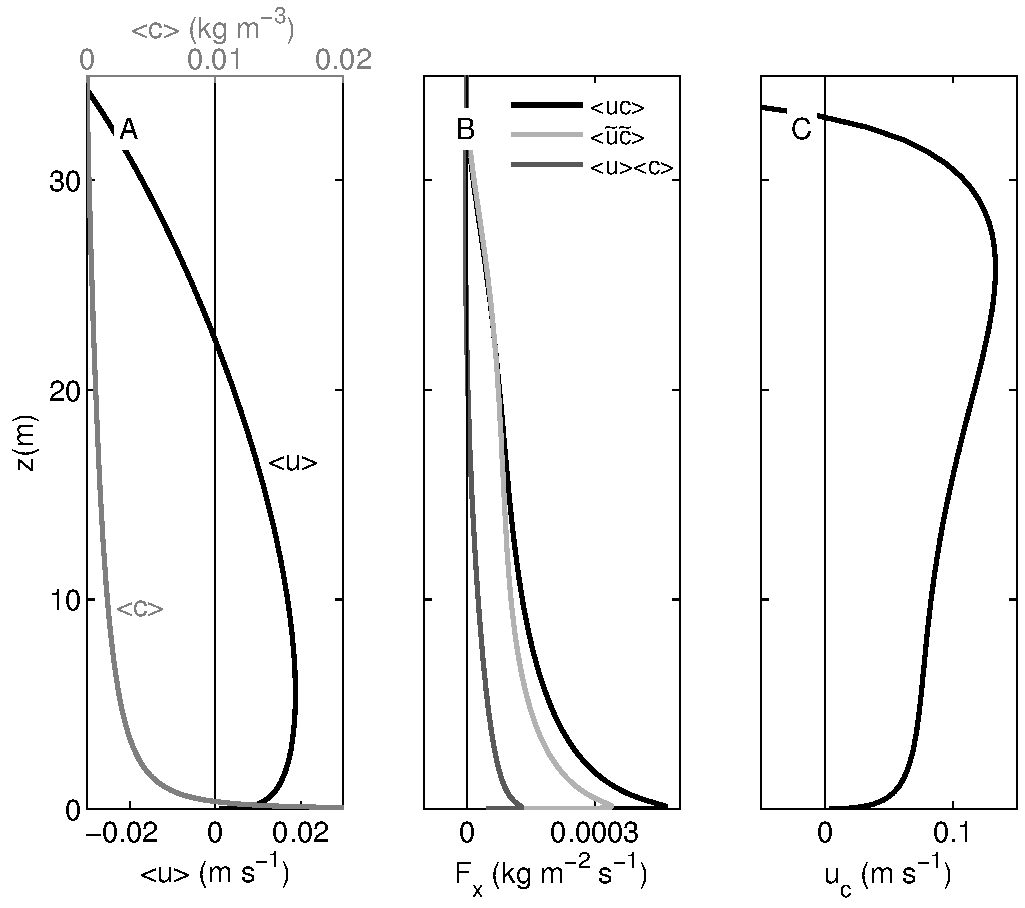
\includegraphics[width=29pc,angle=0]{bilder/profile.pdf}\\
  \caption{Vertical profiles of (a) residual current (black) and
    tidally-averaged SPM concentration (gray), (b) cross-slope
    residual flux, decomposed into contributions from the residual
    current and tidal pumping, and (c) effective cross-slope transport
    velocity computed from \eq{uc}. Note that for clarity only the
    lower part of the domain is displayed. Parameters correspond to
    Case 1 in \tab{params}.}\label{residuals}
\end{figure}
\fig{residuals} shows some tidally-averaged key parameters like the
residual velocity, the SPM concentration, and the cross-slope flux of
SPM, based on the simulation shown in \fig{pannelgrafik}. The residual
currents are of the order of 0.01~m~s$^{-1}$, directed upslope near
the bottom and downslope in the upper part of the BBL
(\fig{residuals}a). In this context, it should be noted that, for
fully periodic conditions and negligible mixing outside the BBL, it
can be mathematically shown that the total cross-slope transport
vanishes for the geometry investigated here
\citep{UmlaufBurchard2011a}:
\begin{equation}
  \label{IntUzero}
   \int_0^\infty \mean{u} \dd z = 0 \point
\end{equation}
This implies that the upslope residual current near the bottom is
exactly compensated by the negative (downslope) residual flow in the
upper part of the BBL.

The tidally-averaged SPM concentration (gray line in \fig{residuals}a)
shows a strong increase towards the bottom, as expected from the
classical Rouse-type balance between sinking and upward turbulent
transport of suspended material. \fig{residuals}b shows that the
residual upslope current in the lower part of the BBL leads to a weak
upslope advection of suspended material. This transport, however, is
negligible in the upper part of the BBL ($z>20$~m), and several times
smaller than the contribution from tidal pumping in the lower
part. This is also mirrored in the effective SPM transport velocity
defined in \eq{uc}, which is several times larger than the residual
current (see \fig{residuals}c). Similar to classical tidal straining,
therefore, we find that tidal pumping is crucial for the total
residual transport of suspended material.

The physical mechanisms inducing tidal pumping in this example are
easily identified from \fig{pannelgrafik}. As discussed above,
sediment concentrations during upslope flow are larger than during
downslope flow due to enhanced erosion and stronger upward mixing of
suspended material. This leads to a positive correlation between
$\tilde{u}$ and $\tilde{c}$, and thus to a residual upslope transport
of suspended material. The magnitude of the transport velocity ($u_c
\sim 0.1$~m~s$^{-1}$) suggests that suspended material is transported
several kilometers upslope during a single tidal cycle in this
example. This supports our main hypothesis that tidal straining in the
BBL near sloping topography constitutes an effective mechanism for the
transport of suspended material across isobaths.
\begin{figure}[h]
  \noindent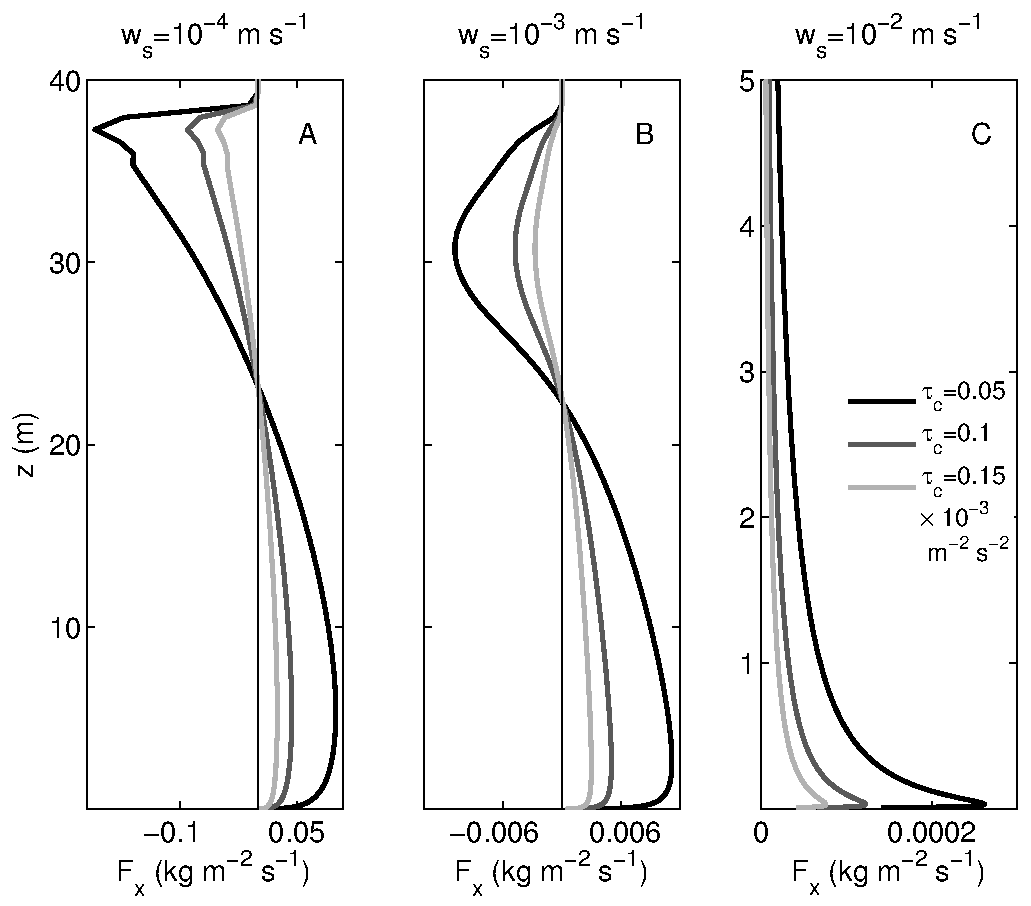
\includegraphics[width=30pc,angle=0]{bilder/tauws.pdf}\\
  \caption{Vertical profiles of residual SPM transports for different
    critical shear stresses (as indicated) and settling velocities:
    (a) $w_s = 10^{-4}\, \text{m s}^{-1}$, (b) $w_s = 10^{-3}\,
    \text{m s}^{-1}$, and (c) $w_s = 10^{-2}\, \text{m s}^{-1}$. All
    other parameters correspond to Case 1 in
    \tab{params}.}\label{compareflux}
\end{figure}

To investigate how this process is affected by the properties of the
suspended material, we compare in \fig{compareflux} the effects of
different sinking speeds and critical shear stresses, leaving all
other parameters unchanged (see Case 1 in \tab{params}). For the
lowest sinking speed ($w_s=10^{-4}$~m~s$^{-1}$), shown in
\fig{compareflux}a, downward sinking of suspended material cannot
compete with upward mixing, and SPM concentrations inside the BBL
therefore fluctuate only marginally around the tidal average
($\tilde{c}/\mean{c} \ll 1$), except in the upper few meters of the
BBL (not shown). In this case, tidal pumping is not effective
($\mean{\tilde{u}\tilde{c}} \ll \mean{u} \mean{c}$), and transports
are largely determined by the two-layer structure of the residual
current shown in \fig{residuals}a.

This situation is contrasted by the case with the highest sinking
speeds ($w_s=10^{-2}$~m~s$^{-1}$), displayed in \fig{compareflux}c,
which is physically similar to the classical tidal pumping mechanism
described already in the context of \fig{residuals}b above: higher SPM
concentrations during the less stratified and more turbulent upslope
flow phase result in a residual upslope transport of suspended
material. Due to the higher sinking velocity compared to
\fig{residuals}b, however, the pumping process is now confined to the
lowest few meters of the water column as shown in \fig{compareflux}c
(note the different vertical scale in this panel).

Physically most interesting is the intermediate case shown in
\fig{compareflux}b, corresponding to a sinking velocity of
$w_s=10^{-3}$~m~s$^{-1}$. Although the vertical structure of the
profile suggests a similarity with the well-mixed case in
\fig{compareflux}a, the underlying processes are entirely
different. Here, the upslope transport of SPM in the lower part of the
BBL (see \fig{compareflux}b) is driven by classical tidal pumping,
analogous to the cases with higher sinking velocities shown in
Figs.\ \ref{residuals}b and \ref{compareflux}c. The downslope
transport observed in the upper part of the BBL, however, is triggered
by a modified (inverse) pumping mechanism resulting from a phase shift
in the SPM concentrations. This is most easily understood from
\fig{pannelgrafik}b, showing that the well-mixed near-bottom layer
reaches its maximum thickness not before the point of flow
reversal. Because newly eroded material is confined to this turbulent
near-bottom layer, maximum SPM concentrations in the upper part of the
BBL are observed with a substantial delay compared to the near-bottom
region (not shown). This phase shift results in a positive correlation
between periods of downslope flow and high SPM concentrations, and
therefore in a residual downslope transport of suspended material in
the upper part of the BBL.

The role of the critical shear stress is investigated in
\fig{compareflux}, where again all other parameters correspond to Case
1 in \tab{params}. According to \eq{defFz}, a lower critical shear
stress leads to a larger erosion flux, and thus, for otherwise
unchanged parameters, to a larger SPM concentration in the water
column. \fig{compareflux} reveals that the net effect is an increase
of the residual SPM fluxes without, however, affecting the basic
mechanisms described above. Similar effects are observed if the bottom
roughness is changed (\fig{roughness}). 
\begin{figure}[h]
  \noindent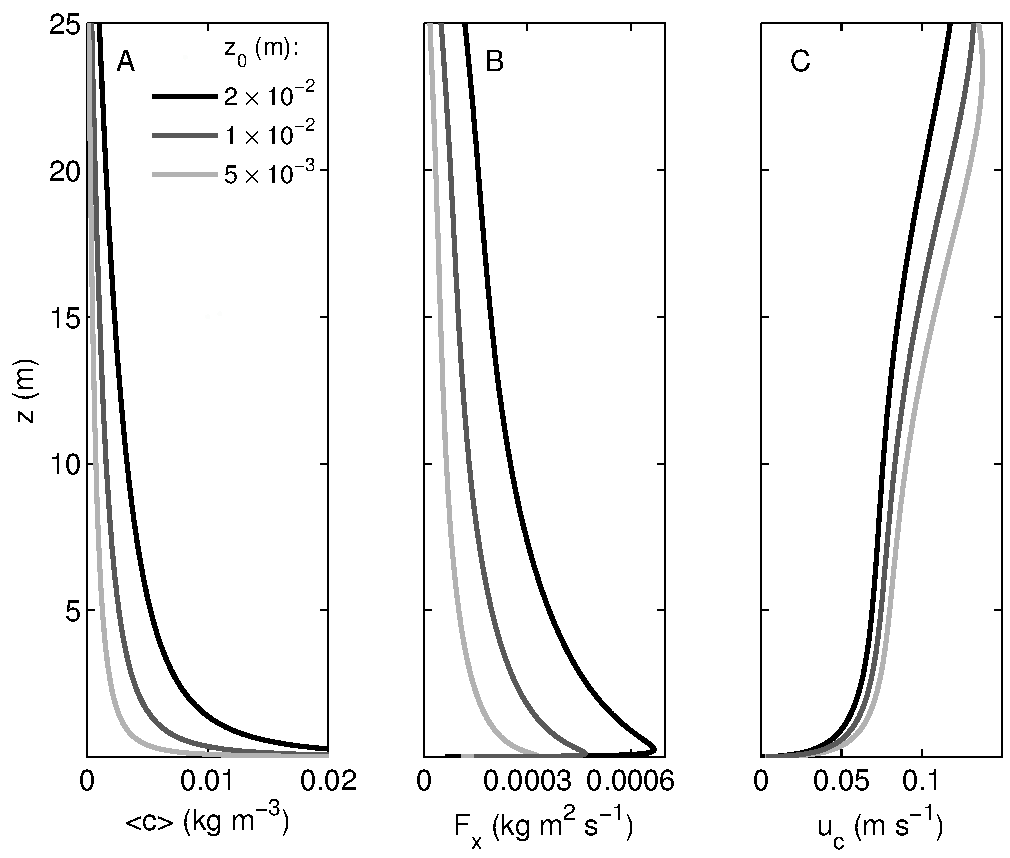
\includegraphics[width=30pc,angle=0]{bilder/bodenz.pdf}\\
  \caption{Profiles of (a) tidally-averaged SPM concentration, (b)
    residual SPM transport, and (c) effective transport velocity for
    different bottom roughnesses (as indicated). All other parameters
    correspond to Case 1 in \tab{params}. Note that, for clarity, only
    the lower part of the domain is displayed.}\label{roughness}
\end{figure}

Reducing or increasing the
bottom roughness by a factor of 2 with respect to the reference case
(Case 1 in \tab{params}), results in significant changes in the bottom
stress, and, therefore, in a modified erosion flux. This results in
strongly altered SPM concentrations and transport rates
(\fig{roughness}a,b) but only in small modifications of the
dynamics. The BBL thickness varies by less than 10\% (not shown), and
the transport velocity by less than 15\% compared to the reference
Case 1 (\fig{roughness}c). Keeping these basic effects of variations
in $\tau_c$ and $z_0$ in mind, we will therefore not investigate the
impact of these parameters in further detail in the following.

\subsection{Supercritical slopes}
The parameters for our second example, used to illustrate the basic
transport mechanisms for subcritical forcing (i.e., supercritical
slopes), are compiled in \tab{params} (Cases 2 and 3). The BBL
resonance period in this case is $T_c \approx 1.1$~h, indicating that
tidal forcing is strongly subcritical. Correspondingly, the slope
angle $\alpha = 0.05$ is more than a factor 10 larger than the
critical slope angle $\alpha_c = 0.0045$.

Despite these differences in forcing, however, the observed flow
patterns exhibit many similarities with Case 1 (subcritical slope)
discussed above. During upslope flow, a gravitationally unstable,
vigorously turbulent near-bottom layer evolves, whereas during
downslope flow, turbulence is suppressed by the generation of stable
stratification (\fig{pannelsupercrit}a,b). 
\begin{figure}[h]
  \noindent\includegraphics[width=30pc,angle=0]{bilder/pannelsupercrit.pdf}\\
  \caption{Temporal variability of (a) velocity, (b) turbulent
    diffusivity, (c) SPM concentration for Case 2, and (d) SPM
    concentration for Case 3. All results represent fully periodic
    conditions (time refers to the start of the simulation). All
    parameters as in \tab{params}.}\label{pannelsupercrit}
\end{figure}

Different from Case 1,
high-frequency oscillations at the BBL resonance period $T_c$ can now
be distinguished in the cross-slope velocities
(\fig{pannelsupercrit}a), however, without significantly modifying the
overall dynamics. More important for the following discussion is the
observation that, due to the stronger tendency for re-stratification,
tidal asymmetries in the turbulent diffusivity and the BBL thickness
are much more pronounced compared to the case with subcritical slope
(\fig{pannelsupercrit}b). E.g., the maximum thickness of the turbulent
BBL varies between $h^\text{up} = 10$~m during upslope flow, and
$h^\text{down} = 3$~m during downslope flow.

\fig{pannelsupercrit}c,d, showing SPM concentrations for two different
sinking speeds, reveals that this asymmetry in BBL thickness strongly
impacts on the vertical SPM distribution.  During upslope flow, SPM is
mixed up higher into the water column, whereas during downslope flow,
most of the suspended material is trapped in the much thinner
turbulent BBL, resulting in extremely high near-bottom SPM
concentrations. After the maximum BBL thickness $h^\text{up}$ during
upslope flow has been reached, the turbulent BBL collapses quickly
during the restratification process
(\fig{pannelsupercrit}b). Particles mixed up during the strongly
turbulent upslope flow phase may therefore remain suspended in the
non-turbulent region above the BBL if their sinking speed is
small. \fig{pannelsupercrit}c shows that this effects leads to
non-zero SPM concentrations above the BBL even after the reversal to
downslope flow.  Quickly sinking particles, on the other hand, will
always be confined to the turbulent BBL (\fig{pannelsupercrit}d).

\begin{figure}[h]
  \noindent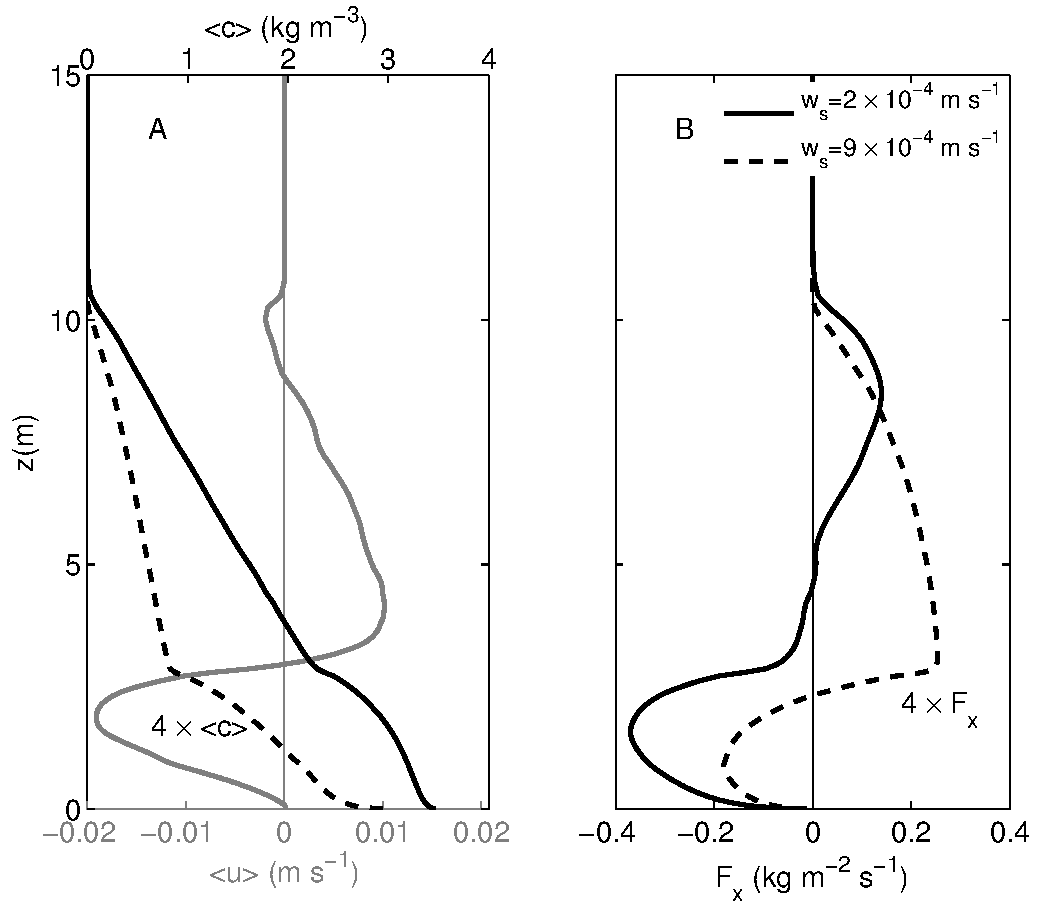
\includegraphics[width=29pc,angle=0]{bilder/Z226profile.pdf}\\
  \caption{Vertical profiles of (a) residual velocity and tidally
    averaged sediment concentration, and (b) residual upslope
    transport for two different sinking speeds as indicated.  For
    better visibility, results for the higher sinking speed ($w_s=9
    \times 10^{-4}$~m~s$^{-1}$) were multiplied by a factor of
    4. Parameters correspond to Cases 2 and 3 in
    \tab{params}.}\label{profsupercrit}
\end{figure}
These extreme tidal asymmetries have a strong impact on the residual
SPM fluxes as illustrated in \fig{profsupercrit}. Both the near-bottom
residual circulation (\fig{profsupercrit}a) and the residual SPM flux
(\fig{profsupercrit}b) suggest a downslope transport of suspended
material in the near-bottom region, which is exactly opposite to the
case with subcritical slope shown in \fig{residuals}. The reversal of
the residual SPM flux close to the bottom ($z<h^\text{down}$) is
easily understood from \fig{pannelsupercrit}c,d, showing that
near-bottom SPM concentrations are much higher during phases of
downslope flow compared to upslope flow. The net effect is a downslope
tidal pumping of suspended material.  The reversal of the near-bottom
residual circulation for super-critical slopes, also evident from
\fig{profsupercrit}a, was already noted by \cite{UmlaufBurchard2011a},
who showed mathematically that this phenomenon occurs if convective
mixing (unstable stratification) during upslope flow dominates
tidally-averaged near-bottom mixing. Similar to the previous examples
for subcritical slopes, however, the contribution of the residual
current to the total residual SPM flux is small compared to the effect
of tidal pumping.

The processes in the upper part of the BBL ($z>h^\text{down}$) are
more similar to classical tidal pumping. Here, SPM concentrations are
larger during periods of upslope flow, when strong turbulence results
in enhanced resuspension and upward mixing of suspended material
(\fig{pannelsupercrit}c,d). While many aspects of this process
resemble the situation for subcritical slopes shown in
\fig{pannelgrafik}, there is one important difference. For quickly
sinking material, the concentration of suspended material is zero
during the downslope flow phase for $z>h^\text{down}$
(\fig{pannelsupercrit}d), resulting in tidal pumping with maximum
efficiency in this region.

The strength and even the direction of the vertically integrated
residual transport are determined by the relative importance of
downslope tidal pumping in the near-bottom region, and upslope tidal
pumping in the region above. The crucial parameter that determines
this interplay is the sinking velocity, as discussed in more detail
below.

\section{Non-dimensional description\label{sec:nondim}}

To investigate the physically relevant parameter space in a systematic
way, it is useful to identify the key non-dimensional parameters that
determine the solutions of the equations described in Section
\ref{sec:geometry}. To this end, we first note that there are eight
dimensional parameters appearing in the equations and boundary
conditions described above. They may be grouped into parameters
related to the properties of the slope ($\alpha$ and $z_0$), the
interior flow ($U$, $\omega$, and $N_\infty$), and the suspended
material ($\alpha_e$, $\tau_c$, and $w_s$). These dimensional
parameters can be combined into five non-dimensional products, with
one possible choice being:
\begin{equation}
  \label{pi}
  \alpha \comma Z = \dfrac{N_\infty}{\omega} \comma R = \dfrac{z_0 \omega}{U} \comma
  P = \dfrac{w_s}{U} \comma T = \dfrac{\tau_c}{U^2} \comma
\end{equation}
where $Z$ is a frequency ratio, $R$ a non-dimensional measure of the
bottom roughness, $P$ a special form of the Rouse number, and $T$ the
non-dimensional critical shear stress. Note that for dimensional
reasons, the erosion parameter $\alpha_e$ does not appear in this or
any other set of non-dimensional products (it is the only parameter
involving the dimension of a mass). 

\subsection{Non-dimensional equations}

In order to understand how these non-dimensional numbers appear in the
governing equations, we start by defining non-dimensional versions of
the time and the slope-normal coordinate:
\begin{equation}
  \label{tznd}
  t^\ast = t \omega \comma  z^\ast = \frac{z \omega}{U} \point
\end{equation}
The dimensional variables appearing in the transport equations in
\eq{ub} and \eq{c} are then non-dimensionalized according to:
\begin{equation}
  \label{paramnd}
  u^\ast = \frac{u}{U}\comma b^\ast = \frac{b}{U N_\infty}\comma
  \tau^\ast = \frac{\tau}{U^2}\comma G^\ast = \frac{G}{U^2 N_\infty}     \comma 
   c^\ast = \frac{cU}{\alpha_e} \comma F_z^\ast = \frac{F_z}{\alpha_e}  \point
\end{equation}
This yields the following non-dimensional equations:
\begin{equation}
  \label{eqs_nondim}
  \begin{array}{rcl}
     \partder{u^\ast}{t^\ast}
    &=& 
    Z \alpha (b^\ast-b_\infty^\ast)  + \cos t^\ast
    - \partder{\tau^\ast}{z^\ast}                   \comma  \\[5mm]
     \partder{b^\ast}{t^\ast}
    &=& 
      - Z \alpha \,  u^\ast- \partder{G^\ast}{z^\ast}                  
                      \comma \\[5mm]
      \partder{c^\ast}{t^\ast} 
     &=& - \partder{}{z^\ast}\left( F_z^\ast
     - P c^\ast \right)          \comma \\[5mm]
  \end{array}
\end{equation}
where we used the special form of the tidal forcing term in
\eq{uinfty}, and assumed mild slopes ($\alpha \ll 1$). It should be
noted that the variables in \eq{paramnd}, although non-dimensional,
are not scaled, i.e.\ terms appearing in \eq{eqs_nondim} are generally
not of order 1.

Only three of the five non-dimensional parameters compiled in \eq{pi}
are seen to appear in \eq{eqs_nondim}. Non-dimensional boundary
conditions, derived from \eq{bound} and \eq{defFz}, are of the form
\begin{equation}
  \label{bc_nondim}
  u^\ast = 0 \comma \partder{b^\ast}{z^\ast} = 0 \comma F_z^\ast =
  \max{ \left\{ \dfrac{\left| \tau_b^\ast \right|}{T}-1,0 \right\} } \quad \text{for} \quad 
z^\ast=0
  \comma
\end{equation}
which reveals that the fourth non-dimensional parameter, the
non-dimensional critical shear stress $T$, appears in the boundary
condition of the erosion model. \cite{UmlaufBurchard2011a} showed that
parameter number five, the roughness number $R$, enters the problem
via the lower boundary condition for the turbulence dissipation
rate. These authors also pointed out that because the
turbulence model does not involve any dimensional constants, no
additional parameters enter the problem.

\subsection{Non-dimensional fluxes}
The total cross-slope transport of suspended material is easily
quantified from the integral of the residual flux defined in \eq{Fx}:
\begin{equation}
  \label{FxInt}
  F_{int} = \int_0^\infty F_x dz \comma
\end{equation}
which can be re-expressed in non-dimensional form as
\begin{equation}
  \label{FxIntND}
  F_{int}^\ast =  \dfrac{\omega}{\alpha_e U} F_{int} 
             = \int_0^\infty F_x^\ast dz^\ast \point
\end{equation}
In order to derive a bulk expression for the effective velocity at
which SPM is transported, it may seem tempting to work with the BBL
average of \eq{uc}. In view of the constraint in \eq{IntUzero},
however, this would eliminate the contribution from the residual
current, which is small but generally not negligible. Also, it should
be noted that, according to \eq{uc}, we find $|u_c| \rightarrow
\infty$ in regions where $\mean{c} \rightarrow 0$. Regions with the
smallest SPM concentrations would therefore provide the largest
contributions to the integral of $u_c$, which therefore cannot be
considered as a sensible bulk measure for the transport velocity.


Here, we use the following alternative approach to define the bulk
transport velocity:
\begin{equation}
  \label{U_c}
  U_c = \dfrac{\int_0^\infty F_x dz}{\int_0^\infty \mean{c} dz} 
  \comma
\end{equation}
which does not exhibit the above problems. The non-dimensional
transport velocity is then defined as $U_c^\ast = U_c / U$. The
quantities $F_{int}^\ast$ and $U_c^\ast$ will be central to the
following analysis of cross-slope SPM transport in non-dimensional
parameter space.

\subsection{Parameter space}
In the following, we investigate the variability of SPM transport
across the physically relevant (non-dimensional) parameter space. All
computations were carried out in dimensional space, and results were
then made non-dimensional as described in the previous sections. Note
that different simulations in dimensional space map onto identical
non-dimensional solutions if they correspond to the same
non-dimensional parameters. We used this fact to test the correctness
of the mathematical and numerical implementation of our model.

Our simulations will be based on the numerical examples discussed in
Section \ref{sec:bbl}, now, however, allowing for a broader range of
variations of the key non-dimensional parameters: the sinking speed
$P$, the stratification parameter $Z$, and the slope angle
$\alpha$. For the non-dimensional sinking speed, we explored the
parameter range $5 \times 10^{-4} \leq P < 5 \times 10^{-2}$ (sampled
with 100 logarithmically spaced intervals), which represents a typical
spectrum of sinking speeds in the ocean
\citep[e.g.,][]{Ferguson2004,vanLeussen1988}. The stratification
parameter $Z$ is varied between $Z=71$ and $Z=224$, corresponding to
one order of magnitude change in the vertical density
gradient. Finally, the slope angle $\alpha$ was varied over the range
$10^{-3} \leq \alpha < 10^{-1}$, which covers virtually all
oceanographically relevant slopes. This range was resolved with 200
logarithmically spaced intervals to account for the large variability
of the SPM fluxes in the vicinity of the critical slope angle (see
below).  

\section{Non-dimensional simulations\label{sec:results}}
In the following, we explore the non-dimensional parameter space
defined above, focusing on the effects of variations in
non-dimensional settling velocity, stratification, and slope angle. To
this end, two groups of simulations with subcritical and supercritical
forcing, respectively, were carried out based on the parameters
summarized in \tab{paramsNDb} (Cases I and II). The non-dimensional parameters
corresponding to Cases 1-3, discussed in the previous sections, are
shown in \tab{paramsNDa} for reference.

\begin{table}[h]
\caption{Non-dimensional parameters corresponding to Cases 1-3 in
  \tab{params}. Note that supercritical forcing corresponds to
  subcritical slopes, and vice-versa.}\label{paramsNDa}
\begin{center}
\begin{tabular}{ccccccc}
\hline\hline
case & forcing & $\alpha$ & $Z$ & $R$ & $P$ & $T$ \\
\hline
1 & supercritical & $2 \times 10^{-3}$ & $71$ & $2.8 \times 10^{-6}$ & $10^{-2}$ & $4 \times 
10^{-4}$ \\
\hline
2 & subcritical & $5 \times 10^{-2}$ & 224 & 
$2.8 \times 10^{-6}$ & $4 \times 10^{-4}$ &  $4 \times 10^{-4}$ \\
\hline
3 & subcritical & $5 \times 10^{-2}$ & 224 & 
$2.8 \times 10^{-6}$ & $2 \times 10^{-3}$ &  $4 \times 10^{-4}$ \\
\hline
\end{tabular}
\end{center}
\end{table}

\begin{table}[h]
\caption{Non-dimensional parameters for the simulations in Section
  \ref{sec:results}. Note that supercritical forcing corresponds to
  subcritical slopes, and vice-versa.}\label{paramsNDb}
\begin{center}
\begin{tabular}{ccccccc}
\hline\hline
case & forcing       & $\alpha$           & $R$                 & $P$               & $T$               \\
\hline
I    & supercritical & $2 \times 10^{-3}$  & $2.8 \times 10^{-6}$ & variable          & $4 \times 10^{-4}$ \\
\hline
II   & subcritical   & $5 \times 10^{-2}$  & $2.8 \times 10^{-6}$ & variable          &  $4 \times 10^{-4}$ \\
\hline
III  & variable      & variable           & $2.8 \times 10^{-6}$ & $10^{-2}$ &  $4 \times 10^{-4}$ \\
\hline
\end{tabular}
\end{center}
\end{table}

\subsection{Supercritical forcing}
\begin{figure}[t]
  \noindent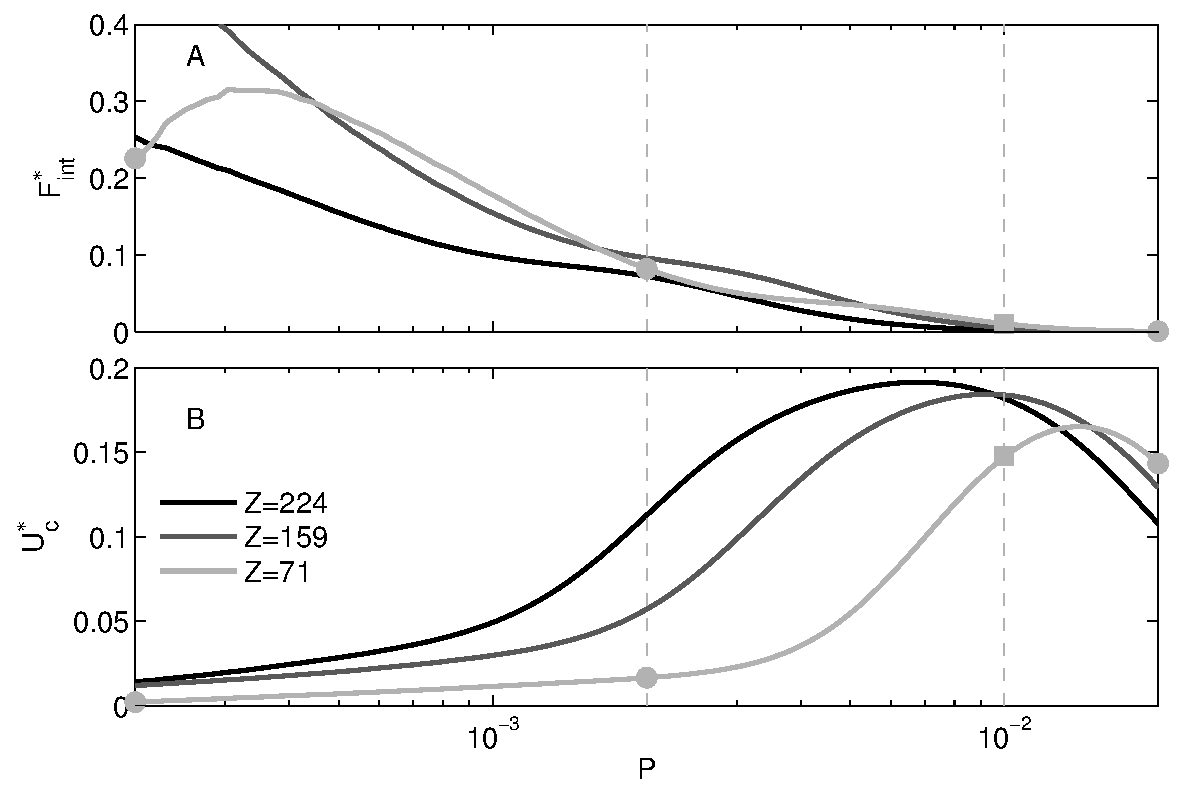
\includegraphics[width=29pc,angle=0]{bilder/subcrit.pdf}\\
  \caption{Variability of (a) non-dimensional integrated SPM
    transport, and (b) non-dimensional bulk transport velocity as a
    function of the non-dimensional sinking speed $P$ and
    stratification parameter $Z$. Parameters correspond to Case I
    (supercritical forcing, see \tab{paramsNDb}).  The square marks
    Case 1 (\tab{paramsNDa}); dots indicate the variations of Case 1
    shown in \fig{compareflux}.}\label{subcrit}
\end{figure}
Non-dimensional transports and transport velocities for the
simulations with supercritical forcing and therefore subcritical
slopes (Case I in \tab{paramsNDb}) are shown in \fig{subcrit}. This
figure reveals, that, for the whole parameter range studied here, the
non-dimensional transport $F_x^\ast$ is positive, suggesting that
suspended material is generally transported in the upslope direction
for subcritical slopes. Transport rates exhibit a decreasing trend for
increasing sinking speeds (\fig{subcrit}a), which is explained, to
first order, by the fact that higher sinking speeds imply smaller SPM
concentrations, and thus smaller net transports. As this effect masks
some of the dynamics, it is, however, more instructive to consider the
behavior of the bulk transport velocity $U_c^\ast$ defined in
\eq{U_c}, which may be viewed as a normalized version of $F_x^\ast$ in
which this direct concentration effect has been
removed. \fig{subcrit}b shows that the dependency of this quantity on
$P$ is similar for all values of $Z$, with low transport velocities
observed for the smallest and largest sinking speeds, respectively,
and a single maximum for moderately large values of the order of
$P=10^{-2}$.

The decay of $U_c^\ast$ for the largest values of $P$ is easily
understood from the fact that in these cases, most of the SPM is
located very close to the bottom, i.e.\ in a region with reduced
velocities due to the effect of bottom friction. In the limiting case
of very large $P$, we would therefore expect a total collapse of the
upslope transport. Small values of $U_c^\ast$ are also found for the
opposite case of very small sinking speeds, where SPM is distributed
nearly homogeneously across the BBL. As discussed above in the context
of \fig{compareflux}a, the transport in this case is determined by the
residual flow rather than tidal pumping, implying that the upslope
transport near the bottom and the downslope transport above nearly
cancel. Although $U_c^\ast$ tends to zero for small $P$, the same is
not true for the transport $F_x^\ast$ (\fig{subcrit}a), which is
largely determined by the strong accumulation of SPM in the BBL due to
the reduced deposition of eroded material. These cases with very small
sinking speeds, however, involve long transients before periodic
conditions are reached, which may rarely be achieved in nature.

For intermediate sinking speeds, \fig{subcrit}b reveals a continuous
increase of $U_c^\ast$ for increasing $P$ until a maximum value of
$U_c^\ast = 0.15-0.2$ is reached, depending on
stratification. Assuming a $M_2$ tide with a typical velocity
amplitude of 1 m~s$^{-1}$, this corresponds to a distance of $\Delta x
= 6.7-8.9$~km over which suspended material is transport upslope
during one tidal cycle. Physically, the increase in $U_c^\ast$ in this
parameter range represents the transition between the situation shown
in \fig{compareflux}b, in which the transports in the upper and lower
parts of the BBL largely compensate, and the more efficient
single-layer transport due to classical tidal pumping in the
near-bottom region as discussed above in the context of
\fig{residuals}b,c and \fig{compareflux}c (these cases are also marked
in \fig{subcrit}). It is remarkable that the maximum transport
velocities for the different values of $Z$ exhibit only a small
variability, despite the fact that the BBL thickness varies by a
factor of 2.5. The overall conclusion from these numerical experiments
is that the transport of SPM is positive (upslope) for supercritical
forcing (subcritical slopes), with the highest transport velocities
found for moderately high sinking speeds as a result of classical
tidal pumping.

\subsection{Subcritical forcing}
\begin{figure}[h]
  \noindent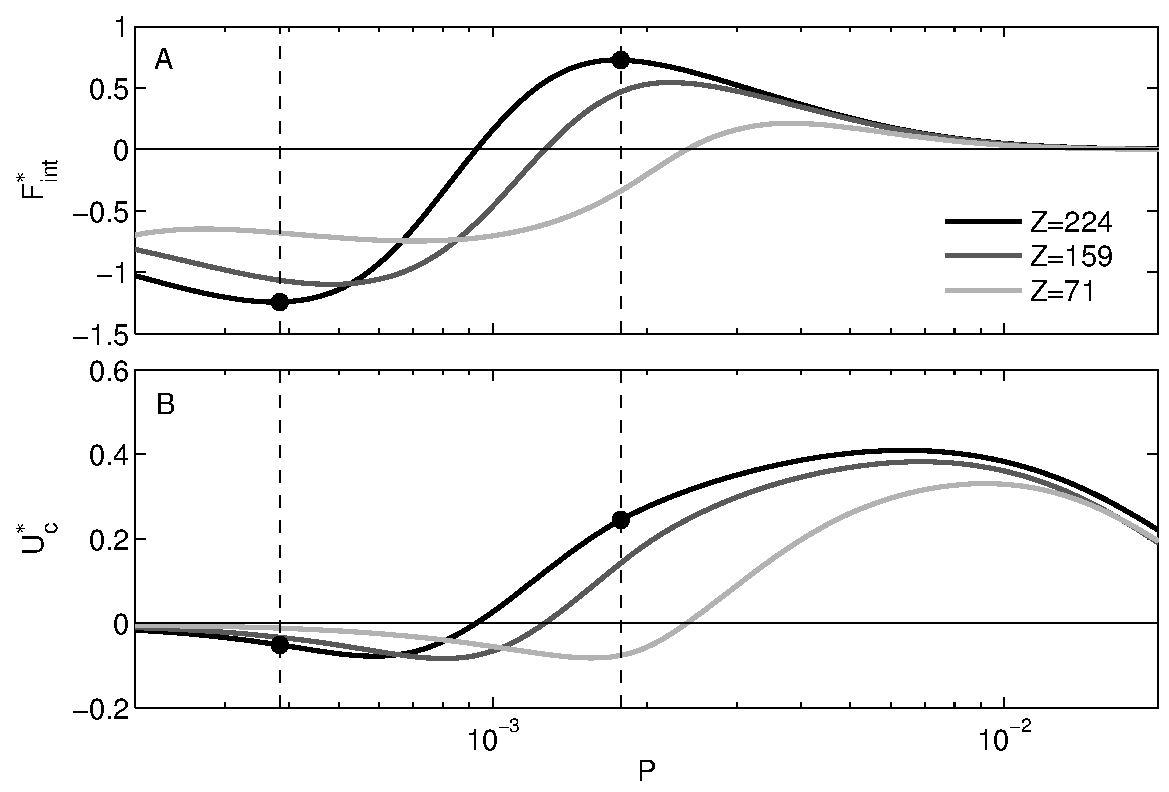
\includegraphics[width=29pc,angle=0]{bilder/supercrit.pdf}\\	
  \caption{As in \fig{subcrit} but now for Case II (subcritical
    forcing, see \tab{paramsNDb}).  Markers indicate Cases 2 and 3
    (\tab{paramsNDa}).}\label{supercrit}
\end{figure}
Results for Case II with subcritical forcing / supercritical slopes
(\tab{paramsNDb}) are displayed in \fig{supercrit}. While the
transports and transport velocities show the same trends, and do so
for the same reasons, as for the cases with supercritical forcing for
very small and large sinking speeds, respectively, there is one
important difference. Below a certain threshold of the sinking speed
$P$ that depends on the stratification parameter $Z$, the transport
now changes direction, and becomes negative (downslope). This
transition was explained in the context of \fig{profsupercrit} as a
result of the decreasing importance of upslope tidal pumping in the
upper part of the domain for decreasing settling velocities. For
slowly sinking material, part of the SPM that has been mixed up high
into the water column during the energetic upslope flow phase remains
suspended in the non-turbulent region above the much thinner BBL
during downslope flow, thus partly compensating the previous upslope
transport. Due to this compensating effect in the upper part of the
domain, the total transport is therefore dominated by the near-bottom
residual transport, which is downslope due to the inverse pumping
mechanism described above.

For quickly sinking material, however, no suspended material is found
in the non-turbulent restratified upper part of the domain that
develops during downslope flow. Tidal pumping above the level of the
thin downwelling BBL is therefore extremely efficient, leading to bulk
transport velocities that reach up to 40\% of the tidal velocity
amplitude (\fig{supercrit}b). We conclude that for both super- and
subcritical forcing, the most efficient upslope transport occurs for
material with moderately large sinking speeds due to classical tidal
pumping. The transport velocities in the subcritical regime, however,
are about twice as large compared to the cases with supercritical
forcing.

\subsection{The effect of the slope angle}
The parameters in all previous examples have been carefully chosen to
insure that the forcing frequency $\omega$ is not in the vicinity of
the critical frequency $\omega_c$ for BBL resonance, where some of the
model assumptions are likely to break down (see above). In the
following analysis, however, we study the model behavior across the
entire range of oceanographically relevant slopes, including the
transition from sub- to supercritical slopes. The parameters for these
simulations correspond to Case III in \tab{paramsNDb}.

\begin{figure}[h]
  \noindent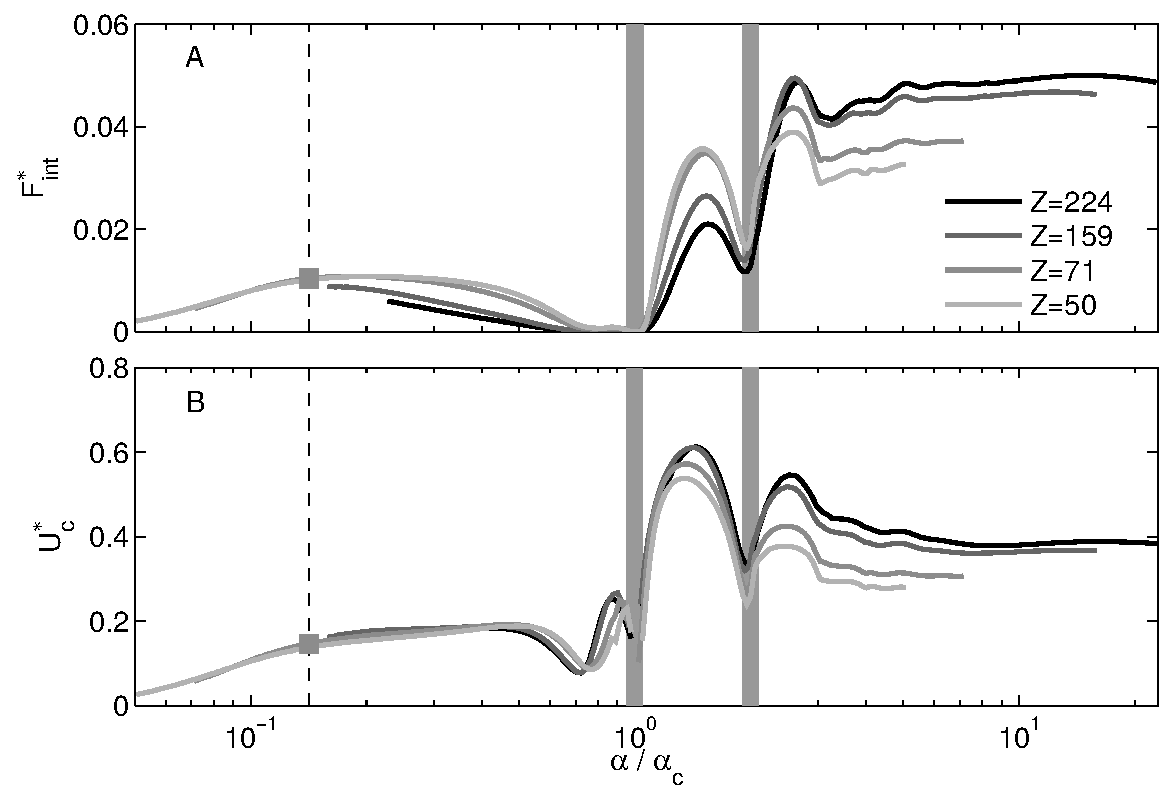
\includegraphics[width=29pc,angle=0]{bilder/alphasoscal.pdf}\\
  \caption{Variability of (a) non-dimensional integrated SPM
    transport, and (b) non-dimensional bulk transport velocity as a
    function of normalized slope angle and non-dimensional
    stratification. Gray-shaded areas indicate the slopes for BBL
    resonance and the first harmonics, respectively. Parameters
    correspond to Case III (variable forcing, \tab{paramsNDb}). The
    marker indicates Case 1 (\tab{paramsNDa}). \label{alphavar} }
\end{figure}
To emphasize the model behavior near critical slopes, in
\fig{alphavar} the slope angle has been normalized by the critical
angle $\alpha_c = \omega/N_\infty$, found from inverting
\eq{omegac}. As shown in the following, the model exhibits a
particular behavior near slopes that correspond to the critical
($\alpha/\alpha_c = 1$) or twice the critical slope ($\alpha/\alpha_c
= 2$), which are therefore indicated in the figure. The
non-dimensional sinking velocity in these examples corresponds to
$P=10^{-2}$, which is close to the efficiency maximum for tidal
pumping as discussed above.

Most obvious from these simulations is the strong increase of both the
SPM transport and the transport velocities at the transition from sub-
to supercritical slopes, consistent with the results discussed in the
preceding sections. Remarkable are the high residual transport
velocities for slightly supercritical slopes ($\alpha \approx 1.4
\alpha_c$), where $U_c$ may reach up to 60\% of the tidal velocity
amplitude. In the immediate vicinity of critical slopes, however,
where the BBL resonantly oscillates at the forcing frequency, the
transport breaks down. A related observations was made by
\cite{UmlaufBurchard2011a}, who pointed out the irreversible upslope
buoyancy flux collapses if the BBL is resonantly
forced. Interestingly, our results also reveal a reduction of the
transport for $\alpha/\alpha_c=2$, which may be understood from the
fact that this case represents the first harmonic, where the BBL
oscillates at exactly twice the forcing frequency.

As suggested already by the results shown in Figs.\ \ref{subcrit} and
\ref{supercrit}, the interpretation of the influence of stratification
is complicated by the strong dependency of the transport rates on the
non-dimensional settling velocity $P$. A robust result, however, seems
to be that transport rates in the strongly supercritical range
($\alpha > 2 \alpha_c$) show a systematic increase with increasing
stratification.


\section{Discussion and conclusions\label{sec:conclusions}}
As one of the most important results, our study suggests that periodic
motions in the vicinity of sloping topography trigger a residual
transport of suspended material that is, for most parameter
combinations, directed upslope. The physical transport mechanisms
resemble classical tidal pumping as described in the context of many
previous studies on SPM transport in estuaries and regions of fresh
water influence \citep[ROFIs,][]{Simpson97a} in the coastal
ocean. However, while classical tidal pumping critically depends on an
externally imposed horizontal density gradient, tidal pumping near
sloping topography only requires: a slope, vertical stratification,
and an oscillating near-bottom current that may be associated with
tidal motions, or, likewise, with any other energetic periodic process
including near-inertial waves, topographically trapped waves, and
internal seiching motions. This combination of factors is nearly
ubiquitous in the ocean and in lakes, and we expect that the same is
true for the new transport mechanism described here.


Our analysis also showed that the residual transport is governed by
five non-dimensional parameters, among them the ratio $P=w_s/U$ of the
sinking speed and the tidal velocity amplitude, which was found to
determine the effectiveness of tidal pumping. The highest transport
velocities are found for values of the order of $P = 10^{-2}$,
i.e. for material with moderately high sinking speeds, assuming a
typical tidal velocity range. For even higher sinking speeds,
suspended material remains in a thin near-bottom layer, where the
transport is inhibited by the effect of bottom friction. For lower
sinking speeds, tidal pumping becomes less efficient.

Beyond the non-dimensional sinking speed $P$, also the roughness
number $R=z_0 \omega / U$, the topographic slope $\alpha$, and the
non-dimensional stratification $Z=N_\infty/\omega$ (the latter two
defining the transition from super- to subcritical forcing) turned out
to be important parameters. A direct comparison of these
non-dimensional parameters with those found in studies of classical
tidal straining in estuaries and ROFIs is, however, complicated by the
fact that the water depth $H$ (one of the key parameters in classical
tidal straining) does not appear in our geometry. Some analogies
between both types of problems can nevertheless be identified, noting
that the key parameters in classical tidal straining are: the Simpson
number, $\text{Si} = H^2 \partial b / \partial x / U^2$, the
unsteadiness number, $\text{Un} = \omega H / U$, and the length scale
ratio $A = z_0/H$
\citep[e.g.,][]{BurchardHetland2010a,Burchardetal2013a}. Recalling
that the (quasi-)horizontal density gradient in our case can be
expressed as $\partial b / \partial x = N_\infty^2 \alpha$ for mild
slopes ($\alpha \ll 1)$, it is easy to show that $\text{Si} \, A^2 =
\alpha Z^2 R^2$ and $\text{Un}\, A = R$, where the left and right hand
sides represent classical and sloping tidal straining,
respectively. Note that some authors identify the velocity scale $U$
with a bulk friction velocity, $U_* \propto U$, which is qualitatively
equivalent.

Our numerical experiments showed that due to the more pronounced tidal
asymmetries for supercritical slopes, SPM transport by tidal pumping
is substantially more efficient than for subcritical $\alpha$. The
sensitivity of the cross-slope fluxes with respect to variations of
the slope angle and ambient stratification implies that the transport
of suspended material near real oceanic slopes, which are in general
neither uniform nor uniformly stratified, exhibits regions of
convergence or divergence of suspended material. This is analogous to
the convergence/divergence of cross-slope buoyancy fluxes discussed by
\cite{Garrett91a}. The results in Section \ref{sec:results} have shown
that the upslope SPM flux strongly increases during the transition
from subcritical to supercritical slopes (see \fig{alphavar}). It may
therefore be speculated that the convergence of suspended material in
the vicinity of critical slopes is balanced by isopycnal intrusions of
SPM towards the interior, possibly promoted by the strong turbulence
usually associated with the critical breaking of internal waves
(\fig{realslopes}a). 
\begin{figure}[t]
  \noindent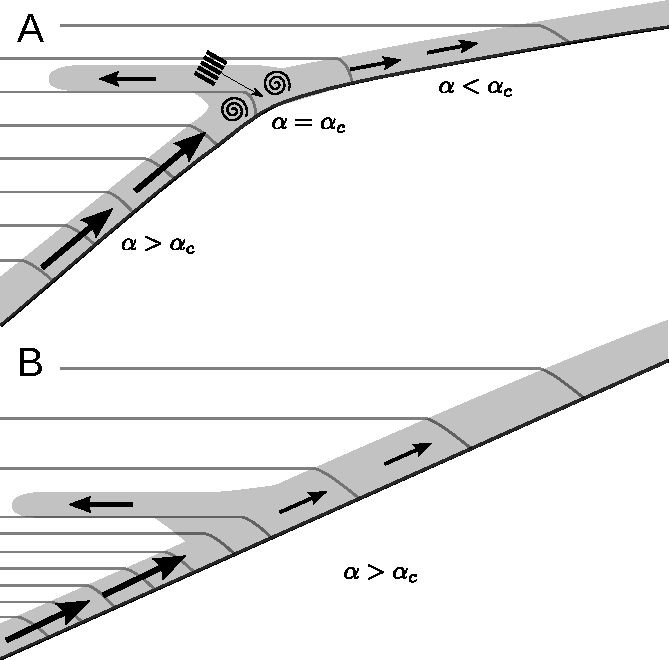
\includegraphics[width=30pc,angle=0]{bilder/outlook.pdf}\\
  \caption{Sketch of possible SPM transport pathways for (a) convex
    topography with varying slope angle and internal-wave breaking at
    the critical slope region as indicated, and (b) changes in
    stratification: a pycnocline below a less stratified water body
    over a supercritical slope. Gray-shaded regions indicate suspended
    material, arrows depict the residual transport of SPM, and gray
    lines denote isopycnals. \label{realslopes} }
\end{figure}
Similarly, for supercritical slopes, a
convergence of upslope transports is expected at the transition from a
region of strong to weak stratification (see \fig{alphavar}), e.g.\ in
the upper part of a pycnocline. As pycnoclines are often regions of
enhanced internal-wave activity, it may be argued that the accumulated
material is resuspended and transported inside the pycnocline towards
the interior (\fig{realslopes}b). These speculations can, however,
only be substantiated with the help of a two- or three-dimensional
modeling approach, which is beyond the scope of our study.

In the present investigation, we have concentrated on the basic
mechanisms of SPM transport due to tidal straining near sloping
topography, ignoring, for simplicity, numerous effects that may become
relevant in more realistic scenarios. These include, besides the
effects of the cross-slope inhomogeneities mentioned above: the effects
of Earth rotation, the role of secondary currents induced by
topographic features like submarine channels or ridges, and the impact
of turbulence on the properties of SPM that all have been shown to
significantly modify the mechanisms of classical tidal straining and
residual SPM transport
\citep[e.g.,][]{MacCreadyGeyer2010,Schulzetal2015a,ScullyFriedrichs2003a}. The
impact of these processes on the dynamics of tidal straining near
sloping topography will have to be clarified in future studies. We
have also emphasized the role of suspended material here but it should be
clear that also bed load transport \citep{vanRijn84a} may provide an
essential contribution to the overall cross-slope transport of
particulate matter. It is likely that the tidal asymmetry in the
bottom stress that we observed in all our simulations (see, e.g.,
\fig{pannelgrafik}e) leads to a residual bed load transport --- but
also this aspect requires a further analysis.
